\documentclass[amsmath,amssymb,aps,prd,10pt,twocolumn,showkeys]{revtex4}
\usepackage{graphicx}
\usepackage{mathtools}
\usepackage{verbatim}
\DeclareMathOperator\erfc{erfc}
\DeclareMathOperator\erf{erf}
\DeclareMathOperator{\sgn}{sgn}
\DeclareMathOperator{\snr}{SNR}
\begin{document}

\title{Complex Analysis of Askaryan Radiation: UHE-$\nu$ Identification and Reconstruction via the Hilbert Envelope of Observed Signals}

\author{Jordan C. Hanson}
\email{jhanson2@whittier.edu}
\affiliation{Department of Physics and Astronomy, Whittier College}
\author{Raymond Hartig}
\affiliation{Department of Physics and Astronomy, Whittier College}
\date{\today}

\begin{abstract}
The detection of ultra-high energy neutrinos (UHE-$\nu$), with enegies above 10 PeV, has been a long-time goal in astroparticle physics.  Autonomous, radio-frequency (RF) UHE-$\nu$ detetectors have been deployed in polar regions.  These detectors rely on the Askaryan effect in ice for the neutrino signal.  The Askaryan effect occurs when the excess negative charge within a high-energy cascade radiates in a dense medium.  UHE-$\nu$ can induce such cascades that radiate in the RF bandwidth above thermal backgrounds.  To identify UHE-$\nu$ signals in future data from Askaryan-class detectors, analytic models of the Askaryan electromagnetic field have been created and compared to simulations and laboratory measurements.  These models have correctly described the Askaryan electromagnetic field, while leaving the effect of the RF detection channels on the field to simulation packages.  In this work, we present a fully analytic Askaryan model that accounts for the effect of an RF detection channel.  First, we derive formulas for the observed voltage trace, and for the Hilbert envelope of the trace.  Second, we match the analytic model to data computed for a detector with a single string of eight RF detection channels in NuRadioMC, a key Monte Carlo toolset in UHE-$\nu$ detection.  For UHE-$\nu$ signals above RF thermal backgrounds, we find correlation coefficients in excess of $0.95$.  Third, 92\% of UHE-$\nu$ signals pass a correlation threshold of 0.438, while all but 0.95 out of $1.57 \times 10^8$ RF thermal triggers are rejected.  At a thermal trigger rate of 1 Hz, this corresponds to 5 years of continuous operation.  Finally, we reconstruct the logarithm of the UHE-$\nu$ cascade energy.
\end{abstract}

\keywords{Ultra-high energy neutrino; Askaryan radiation; Mathematical physics}

\maketitle

\section{Introduction}

Cosmic neutrinos with energies up to 100 PeV have been detected by the IceCube and KM3NeT collaborations \cite{10.1126/science.1242856,aartsen2013first-bff,collaboration2016observation-03b,collaboration2018neutrino-2a0,collaboration2021detection-6fa,collaboration2022evidence-a08,collaboration2023observation-08b,collaboration2025observation-22f}. Previous analyses indicate that the discovery of neutrinos above 5 PeV to 20 EeV will  require large Askaryan-class detectors \cite{10.1103/physrevd.98.062003}.  Neutrinos with energies in the EeV range could potentially reveal the source of ultra-high energy cosmic rays (see sections 3.1-3.3 of \cite{10.48550/arxiv.2008.04323}).  Further, studying electroweak interactions at these energies is impossible on Earth, and Askaryan-class neutrino detectors provide new data (see section 3.4 of \cite{10.48550/arxiv.2008.04323}).

This work is the first application of the Hanson and Hartig (HH) model for the purposes of reconstruction.


\section{Units, Definitions, and Conventions}
\label{sec:unit}

\begin{itemize}
\item The result for $\mathcal{E}_{r*s}(t)$, Eqs. \ref{eq:final} and \ref{eq:final2}, depends on the model for $s(t)$, Eq. \ref{eq:s}.  Equation \ref{eq:s} is a simplified version of Eq. 28 in the analysis presented by Hanson and Hartig (HH) \cite{PhysRevD.105.123019}.  The $E_0$ simply represents all time-independent amplitude factors.  The full expression for $s(t)$ is
\begin{equation}
r\vec{E}(t_{\rm r},\theta) = -\frac{E_0\omega_0 \sin(\theta)}{8\pi p}t_{\rm r}e^{-\frac{t_{\rm r}^2}{4p}+p\omega_0^2}\erfc(\sqrt{p}\omega_0) \label{eq:s_full}
\end{equation}
\begin{table*}
\begin{tabular}{| c | c | c |} \hline
\textbf{Variable} & \textbf{Definition} & \textbf{Units}\\ \hline
$c$ & speed of light in medium & m ns$^{-1}$ \\ 
$r$ & distance to cascade peak & m \\
$t_{\rm r}$ & $t-r/c$ & ns \\
$\theta_{\rm C}$ & Cherenkov angle & radians \\ 
$\theta$ & viewing angle from cascade axis & radians \\ 
$a$ & longitudinal cascade length (see \cite{10.1103/physrevd.65.016003}) & m \\ 
$n_{max}$ & max excess cascade particles (see \cite{10.1103/physrevd.65.016003})  & none \\
$E_{\rm 0}$ & $\propto n_{\rm max}a$ (see \cite{10.1103/physrevd.65.016003}) & V GHz$^{-2}$ \\
$p$ & $\frac{1}{2}(a/c)^2 \left(\cos\theta - \cos\theta_C\right)^2$ (see \cite{PhysRevD.105.123019}) & ns$^2$ \\ 
$\omega_{\rm 0}$ & $\sqrt{\frac{2}{3}} (c\sqrt{2\pi}\rho_{\rm 0})/(\sin\theta)$ (see \cite{10.1016/j.astropartphys.2017.03.008}) & GHz \\
$\sqrt{2\pi}\rho_{\rm 0}$ & lateral ICD width (see \cite{10.1016/j.astropartphys.2017.03.008}) & m$^{-1}$ \\ \hline
\end{tabular}
\caption{\label{tab:param} things.}
\end{table*}

The parameters of Eq. \ref{eq:s_full} are shown in Tab. \ref{tab:param}.  Though Ralston and Buniy (RB) \cite{10.1103/physrevd.65.016003} used $c$ for the vaccuum value of the speed of light, the formulae for $r \vec{E}$ presented in \cite{10.1103/physrevd.65.016003} refer to the wavenumber $k$ in the medium, which is proptional to the index of refraction. Thus, the use of $c$ in this work refers to the speed of light in the medium.  For example, a phase factor of $\exp(j k r)$ could also be written $\exp(j r \omega/c)$, if $c$ refers to the value in the medium.  The distance $r$ is between the observer and the radiating charge at the cascade peak.  The longitudinal length over which $\Delta r < \lambda$, the RF wavelength in ice, is named the \textit{coherence zone} $\Delta z_{\rm coh}$ in the RB model.  The $\Delta z_{\rm coh}$ is limited by what RB call the ``acceleration argument,'' that $r(t)$ is accelerating while keeping $\Delta r < \lambda$.

The longitudinal cascade length, $a$, is set by the cascade physics.  The ratio $\eta = (a/\Delta z_{\rm coh})^2$ corresponds to the far-field limit as $\eta \to 0$, but this is not a requirement of the RB model.  In fact, the RB equations are valid when $\eta > 1$.  Hanson and Connolly (JCH+AC) have shown that $\eta$ corresponds to low-pass filter with cutoff $\omega_{\rm C}$ that limits the RF emissions, $\eta = \omega/\omega_{\rm C}$ \cite{10.1016/j.astropartphys.2017.03.008}.  JCH+AC also studied $\omega_{\rm C}$ over the frequency and $a$ parameter space, because this parameter space is relevant for the LPM effect.

The time $t$ is the independent variable of the inverse Fourier transform of the equations in \cite{10.1103/physrevd.65.016003}. The delayed time is $t_{\rm r} = t-r/c$.  The Cherenkov angle $\theta_{\rm C}$ is set by the index of refraction, $n$, via $\cos\theta_{\rm C} = 1/n$.  The value for the RF bandwidth in solid ice ($n=1.78$) is 55.8 degrees.  More detail on the index of refraction in polar ice is given in \cite{Barwick:2018497,ALLISON201963}.  The viewing angle $\theta$ is measured relative to the cascade axis, and Askaryan radiation is concentrated for $\theta \approx \theta_{\rm C}$.  The $n_{\rm max}$ parameter is the maximum excess negative cascade charge, and the overall RF amplitude, $E_{\rm 0}$, is propotional to $n_{\rm max} a$.

JCH+AC and Hanson and Hartig (HH) demonstrate how the cutoff frequency $\omega_{\rm 0}$ is related to the instantaneous charge distribution (ICD) and the cascade form factor \cite{10.1016/j.astropartphys.2017.03.008,PhysRevD.105.123019}.  Monte Carlo simulations have shown that the lateral dependence of the ICD is, to first order, exponentially distributed \cite{zhs,PhysRevD.105.123019}.  In JCH+AC, characterizing the lateral component of the ICD as $\exp(-\sqrt{2\pi}\rho_0 \rho)$ led to an elegant expression for the ICD form factor, $\widetilde{F}(\omega)$.

Hanson and Hartig (HH) have shown that the parameter $p$ is related to $\sigma_t$ \cite{PhysRevD.105.123019}:

\begin{equation}
\sigma_t = \sqrt{2p} \label{eq:pulse_width}
\end{equation}

The authors of \cite{PhysRevD.105.123019} have shown that, because $\cos\theta - \cos\theta_{\rm C} \approx -\sin\theta_{\rm C}(\theta-\theta_{\rm C})$ to first order in $\Delta\theta=(\theta-\theta_{\rm C})$, $p \propto \Delta\theta^2$ to second order, and 

\begin{equation}
a\Delta\theta = \frac{c \sigma_t}{\sin\theta_{\rm C}} \label{eq:uncert}
\end{equation}

Qualitatively, this notion was identified by RB in Sec. III of \cite{10.1103/physrevd.65.016003}.  HH analyzed the relationship between $a$, the cascade energy $E_{\rm C}$ and the critical energy $E_{\rm crit}$ for electromagnetic and hadronic cascades \cite{PhysRevD.105.123019}.  Let $E_{\rm C}/E_{\rm crit} = \Lambda$.  Assuming the Greisen and Gaisser-Hillas parameterizaions for electromagnetic and hadronic cascades, respectively, HH found the relationship

\begin{align}
a &= c_{\rm em} \sqrt{\ln\Lambda} \label{eq:em} \\
a &= c_{\rm had} \sqrt{\ln\Lambda} \label{eq:had}
\end{align}

\begin{equation}
\frac{\sigma_{\ln\Lambda}}{\ln\Lambda} = 2\left(\frac{\sigma_a}{a}\right) \label{eq:a_err}
\end{equation}

Equation \ref{eq:a_err} corresponds to Eq. 42 in \cite{PhysRevD.105.123019}, and has been corrected for units.  Equations \ref{eq:pulse_width}-\ref{eq:a_err} imply measurements of $a$ and $\Delta\theta$ lead to a measurement of the logarithm of the cascade energy $\ln\Lambda$, and that the relative error in $\ln\Lambda$ is proportional to the relative error in $a$.
\end{itemize}

\section{Collection of Main Results}
\label{sec:onc}

Here is a list of the basic results and ideas for this paper.

\begin{itemize}
\item Let the signal model $s(t)$ be
\begin{equation}
s(t) = -E_0 t e^{-\frac{1}{2}\left(t/\sigma_t\right)^2} \label{eq:s}
\end{equation}
This is the off-cone field equation from \cite{PhysRevD.105.123019}.  The parameter $\sigma_{\rm t}$ is the pulse width, and it depends two quantities: the longitudinal length of the UHE-$\nu$-induced cascade, and the angle at which the cascade is observed relative to the Cherenkov angle.  The parameter $E_0$ is the amplitude normalization, and it depends on two parameters: $\sigma_{\rm t}$, and $\omega_{\rm 0}$, the cutoff frequency from the cascade form factor.  In Sec. \ref{sec:onc}, $E_0$ and $\sigma_t$ will be treated as constants, since neither depends on time.
\item Let $\widehat{s}(t)$ represent the Hilbert transform of $s(t)$.  The \textit{analytic signal} of $s(t)$ is
\begin{equation}
s_{\rm a}(t) = s(t) + j \widehat{s}(t)
\end{equation}
The magnitude of the analytic signal, $|s_a(t)|$, is the \textit{envelope} of the signal.  The Hilbert transform $\widehat{s}(t)$ is equivalent to the convolution of $s(t)$ and the tempered distribution $h(t) = 1/(\pi t)$.
\item Let $S(f)$ be the Fourier transform of $s(t)$.  The Fourier transform of the analytic signal is
\begin{equation}
\mathcal{F}\lbrace s_{\rm a}(t) \rbrace_{f} = S_{\rm a}(f) = S(f)(1+\sgn{f}) \label{eq:sa_1}
\end{equation}
The sign function, $\sgn$ gives $-1$ if $f<0$, $0$ if $f=0$, and $1$ if $f>1$.
\item Taking the inverse Fourier transform of Eq. \ref{eq:sa_1}, the analytic signal may be written in terms of $S(f)$:
\begin{equation}
s_{\rm a}(t) = 2\int_{0}^{\infty} S(f) e^{2\pi j f t} df \label{eq:sa_2}
\end{equation}
\item The Fourier transform of Eq. \ref{eq:s} is
\begin{equation}
S(f) = E_0 \sigma_t^3 (2\pi)^{3/2} j f e^{-2\pi^2 f^2 \sigma_t^2}
\end{equation}
\item Using the gaussian spectral width $\sigma_{\rm f}$ from \cite{10.1016/j.astropartphys.2017.03.008}, and the guassian width of $s(t)$ from \cite{PhysRevD.105.123019}, it was shown in \cite{PhysRevD.105.123019} that the uncertainty principle holds for off-cone signals:
\begin{equation}
\sigma_t \sigma_f \geq \frac{1}{2\pi}
\end{equation}
The equality is reached in the limit the far-field parameter limits to zero: $\eta \to 0$.  This makes the signal spectrum
\begin{equation}
S(f) = E_0 \sigma_t^3 (2\pi)^{3/2} j f e^{-\frac{1}{2}\left(f/\sigma_f\right)^2} \label{eq:spec}
\end{equation}
Inserting $S(f)$ into Eq. \ref{eq:sa_2}, $s_{\rm a}(t)$ is
\begin{equation}
s_{\rm a}(t) = \frac{E_0 \sigma_t^3 (2\pi)^{3/2}}{\pi} \frac{d}{dt}\int_0^{\infty} e^{-\frac{1}{2}\left(f/\sigma_f\right)^2} e^{2\pi j f t} df \label{eq:sa_3}
\end{equation}
\item Let $k^2/4 = \frac{1}{2}\left(f/\sigma_f\right)^2$, and $x = t/(\sqrt{2}\sigma_t)$.  Equation \ref{eq:sa_3} can be broken into real and imaginary parts:
\begin{align}
s_{\rm a}(t) &= \frac{E_0 \sigma_{\rm t}}{\sqrt{2\pi}}\frac{dI}{dx} \\
\Re\lbrace I \rbrace &= \int_0^{\infty} e^{-k^2/4}\cos(kx) dk \\
\Im\lbrace I \rbrace &= \int_0^{\infty} e^{-k^2/4}\sin(kx) dk
\end{align}
The real part of $I$ is even, so it can be extended to $(-\infty,\infty)$ if it is multiplied by $1/2$.  The result is
\begin{equation}
\Re\lbrace I \rbrace = \sqrt{\pi} e^{-x^2}
\end{equation}
The imaginary part of $I$ is proportional to \textit{Dawson's integral, $D(x)$} \cite{NIST:DLMF}:
\begin{equation}
\Im\lbrace I\rbrace = 2 D(x)
\end{equation}
\item The overall analytic signal, $s_a(t)$, is
\begin{equation}
s_a(t) = -E_0 \left(t e^{-\frac{1}{2}\left(t/\sigma_t\right)^2} - \frac{2 j\sigma_t}{\sqrt{2\pi}} \frac{dD(x)}{dx}\right) \label{eq:sa_4}
\end{equation}
The signal envelope is $|s_a(t)|$.  It is important to note that, though $D(x)$ is not evaluated analytically, a high-precision algorithm for computing $D(x)$ was given in \cite{10.1063/1.4822832}.  Note that $s_a(0) \neq 0$, since $dD(x)/dx = 1 - 2x D(x)$.
\item Signal data in detectors designed to observe Askaryan pulses is equivalent to the convolution of the signal and detector response functions.  Signal models are convolved with measured detector responses to create \textit{signal templates}.  Signal templates are cross-correlated with observed data to identify UHE-$\nu$ signals.  The oscillations of signal templates and observed data can introduce various uncertainties when cross-correlated.  This problem intensifies when the signal-to-noise ratio between Askaryan pulse data and thermal noise decreases.  To reduce these uncertainties, the Hilbert envelope of observed signals is used in cross-correlations instead of the original signals.  We seek an analytic equation for the Hilbert envelope of the data.  That is, we seek the envelope of the convolution of the analytic signal model with a typical detector response.  The RLC damped oscillator is a standard circuit model for the RF dipole antennas used in RNO-G and the proposed IceCube Gen2 \cite{10.1103/PhysRevD.85.062004,10.1088/1748-0221/16/03/p03025,10.48550/arxiv.2008.04323}.
\item There are two paths to calculating the final result.  The first option involves three steps.  First, the detector response, $r(t)$ is convolved with $s(t)$.  Second, the analytic signal of the result is found.  Third, the magnitude of the analytic signal is computed, which can be compared to envelopes of observed signals.  The second option involves computing the envelope of the convolution of $r(t)$ with $s(t)$ directly from $s_a(t)$ and $r_a(t)$.
\item Let $s(t) * r(t)$ represent the convolution of $s(t)$ and $r(t)$.  Let the envelope of the convolution be $\mathcal{E}_{s * r}(t)$.  $\mathcal{E}_{s * r}(t)$, $s_a(t)$, and $r_a(t)$ are related by
\begin{equation}
\mathcal{E}_{s * r}(t) = \frac{1}{2}| s_a (t) * r_a(t)| \label{eq:awesome}
\end{equation}
The proof of Eq. \ref{eq:awesome} is based on two ideas.  First, the Hilbert transform of a function $s(t)$ is equivalent to convolving it with the ``tempered distribution'' $h(t) = 1/(\pi t)$.  Second, computing the Hilbert transform twice yields the original function, multiplied by $-1$: $h * h * s = -s$.  Given the definitions of the analytic signal and the Hilbert transform,
\begin{align}
(s * r)_a (t) &= s * r + j ~ \widehat{s*r} \\
\mathcal{E}_{s * r}(t) &= | s * r + j s * r * h|
\end{align}
However,
\begin{align}
r_a * s_a &= (r + j \hat{r}) * (s + j \hat{s}) \\
r_a * s_a &= r * s + j r * \hat{s} + j \hat{r} * s - \hat{r} * \hat{s} \\
r_a * s_a &= r * s - r * h * s * h + 2 j h * r * s \\
r_a * s_a &= r * s - h * h * r * s + 2 j h * r * s \\
r_a * s_a &= 2 r * s + 2 j h * r * s
\end{align}
Multiplying both sides $1/2$ and taking the magnitude completes the proof:
\begin{equation}
\frac{1}{2} |r_a * s_a| = |r * s + j h * r * s| = \mathcal{E}_{s * r}(t) \\
\end{equation}
\item Assume that a signal arrives in an RLC damped oscillator at $t=0$.  For $t\geq 0$, the impulse response and corresponding analytic signal are
\begin{align}
r(t) &= R_0 e^{-2 \pi \gamma_f t} \cos(2\pi f_0 t) \label{eq:r} \\
r_a(t) &= R_0 e^{-2 \pi \gamma_f t} e^{2\pi j f_0 t} \label{eq:ra}
\end{align}
The parameters $\gamma_f$ and $f_0$ are the \textit{decay constant} that corresponds to the \textit{fall time} of the output signal, and the resonance frequency.  Note that the envelope of $r(t)$, $|r_a(t)|$, is $R_0 \exp(-2 \pi \gamma_f t)$, as expected.  To prove Eq. \ref{eq:ra}, first compute the Fourier transform of $r(t)$:
\begin{align}
R(f) &= \frac{R_0}{4\pi j} \left( \frac{1}{f - z_{+}} + \frac{1}{1- z_{-}} \right) \\
z_{+} &= f_0 + j \gamma_f \\
z_{-} &= -f_0 + j \gamma_f
\end{align}
Given Eq. \ref{eq:sa_2}, the procedure to find $r_a(t)$ is to multiply the \textit{negative} frequency components by 0 and the \textit{positive} frequency components by 2, and take the inverse Fourier transform.  The inverse Fourier transform may be completed by extension to the complex plane using the upper infinite semi-circle as a contour, and applying Jordan's lemma.  The residue from the pole at $z_{+}$ drives the final result. (Check the sign of time here, to ensure that it is positive).
\item The goal is now to apply Eq. \ref{eq:awesome} by convolving $s_a(t)$ with $r_a(t)$.  The calculation may be split into two parts: $r_a(t) * \Re\lbrace s_a(t) \rbrace$, and $r_a(t) * \Im\lbrace s_a(t) \rbrace$.  Let $u(t)$ represent the Heaviside step function.  Starting with $r_a(t) * \Re\lbrace s_a(t) \rbrace$:
\begin{multline}
r_a(t) * \Re\lbrace s_a(t) \rbrace = \\ R_0 e^{2\pi j f_0 t} e^{-2\pi\gamma t} u(t) * \left(-E_0 t e^{-\frac{1}{2}\left(t/\sigma_t\right)^2}\right)
\end{multline}
Let $x=t/(\sqrt{2}\sigma_t)$, $y=\tau/(\sqrt{2}\sigma_t)$, and $z = (2\pi j f_0 - 2\pi\gamma)\sqrt{2}\sigma_t$.  Changing variables while accounting for the relationship between $u(t)$, $x$, and $y$, gives
\begin{multline}
r_a(t) * \Re\lbrace s_a(t) \rbrace = \\ -2R_0 E_0 \sigma_t^2 \int_{-\infty}^{x} e^{z(x-y)} y e^{-y^2} dy
\end{multline}
Note that the units for the convolution of $r(t)$ and $s(t)$ correspond to $R_0 E_0 \sigma_t^2$.  Let $u = x-y$, so that $du = -dy$. The result is
\begin{equation}
r_a(t) * \Re\lbrace s_a(t) \rbrace = 2R_0 E_0 \sigma_t^2\left(\frac{dI(x,z)}{dz}-xI(x,z)\right)
\end{equation}
where
\begin{equation}
I(x,z) = \int_0^{\infty} e^{zu} e^{-(u-x)^2} du
\end{equation}
Let $b = x+\frac{1}{2} z$. Completing the square in the exponent and substituting $k = u-b$ gives
\begin{multline}
I(x,z) = e^{-x^2} e^{b^2} \int_{-b}^{\infty} e^{-k^2} dk \\ = \frac{\sqrt{\pi}}{2} e^{-x^2} e^{b^2} \erfc(-b)
\end{multline}
Let $b = jq$, and $w(q)$ be the \textit{Faddeeva function} \cite{NIST:DLMF}.  The integral becomes
\begin{equation}
I(x,z) = \frac{\sqrt{\pi}}{2} e^{-x^2} w(q)
\end{equation}
The chain rule is required to find $dI/dz$:
\begin{equation}
\frac{dI}{dz} = \frac{dI}{dq}\frac{dq}{dz} = -\left(\frac{j}{2}\right)\frac{dI}{dq}
\end{equation}
The final result is
\begin{multline}
r_a(t) * \Re\lbrace s_a(t) \rbrace = \\ -\sqrt{\pi} R_0 E_0 \sigma_t^2 \left(x e^{-x^2} w(q) + \left(\frac{j}{2}\right) e^{-x^2} \frac{dw(q)}{dq} \right) \label{eq:Re_result}
\end{multline}
\item Turning to the convolution of $r_a(t)$ with $\Im(s_a)$,
\begin{multline}
r_a(t) * \Im\lbrace s_a(t) \rbrace = \\ \left(R_0 e^{2\pi j f_0 t} e^{-2\pi \gamma t} u(t)\right) * \left(\frac{2 E_0 \sigma_t^2}{\sqrt{\pi}}\frac{dD(t/\sqrt{2}\sigma_t)}{dt} \right)
\end{multline}
Note that $f'(t) * g(t) = f(t) * g'(t) = (f(t) * g(t))'$.  Thus,
\begin{multline}
r_a(t) * \Im\lbrace s_a(t) \rbrace = \\ \frac{2}{\sqrt{\pi}} R_0 E_0 \sigma_t^2 \frac{d}{dt}\left(e^{2\pi j f_0 t}e^{-2\pi\gamma t} u(t) * D(t/\sqrt{2}\sigma_t) \right)
\end{multline}
Accounting for the step function in the convolution gives
\begin{multline}
r_a(t) * \Im\lbrace s_a(t) \rbrace = \\ \frac{2}{\sqrt{\pi}} R_0 E_0 \sigma_t^2 \frac{d}{dt} \int_{-\infty}^{t} e^{(2\pi j f_0 - 2\pi\gamma)(t-\tau)}D(\tau/\sqrt{2}\sigma_t)d\tau
\end{multline}
Adopting the earlier definitions of $x$, $y$, and $z$ gives
\begin{multline}
r_a(t) * \Im\lbrace s_a(t) \rbrace = \\ \frac{2}{\sqrt{\pi}} R_0 E_0 \sigma_t^2 \frac{d}{dx} \int_{-\infty}^{x} e^{z(x-y)} D(y) dy
\end{multline}
Using the fundamental theorem of calculus, and the limiting cases of $D(x)$, 
\begin{multline}
r_a(t) * \Im\lbrace s_a(t) \rbrace = \\ \frac{2}{\sqrt{\pi}} R_0 E_0 \sigma_t^2 \left(D(x) + z\int_{-\infty}^{x} e^{z(x-y)} D(y) dy \right)
\end{multline}
Let $u = x-y$, $z=-k$, and note that $D(x)$ is an odd function.  These substitutions give
\begin{multline}
r_a(t) * \Im\lbrace s_a(t) \rbrace = \\ \frac{2}{\sqrt{\pi}} R_0 E_0 \sigma_t^2 \left(D(x) + k\int_{0}^{\infty} e^{-ku} D(u-x) du \right)
\end{multline}
The remaining integral is the Laplace transform of the shifted Dawson function, $\mathcal{L}\lbrace D(u-x)\rbrace_k$.  The final result is
\begin{equation}
r_a(t) * \Im\lbrace s_a(t) \rbrace = \\ \frac{2}{\sqrt{\pi}} R_0 E_0 \sigma_t^2 \left(D(x) + k\mathcal{L}\lbrace D(u-x)\rbrace_k\right) \label{eq:Im_result}
\end{equation}
Though a closed analytic form for $\mathcal{L}\lbrace D(u-x)\rbrace_k$ is elusive, finishing this calculation through numerical integration is straightforward.
\item Combining Eq. \ref{eq:Re_result} and Eq. \ref{eq:Im_result} gives $r_a(t) * s_a(t)$, since
\begin{equation}
r_a(t) * s_a(t) = r_a(t) * \Re\lbrace s_a(t)\rbrace + j r_a(t) * \Im\lbrace s_a(t)\rbrace
\end{equation}
which yields
\begin{multline}
r_a(t) * s_a(t) = \\ -\sqrt{\pi} R_0 E_0 \sigma_t^2 \left(x e^{-x^2} w(q) + \left(\frac{j}{2}\right) e^{-x^2} \frac{dw(q)}{dq} \right) + \\ \frac{2j}{\sqrt{\pi}} R_0 E_0 \sigma_t^2 \left(D(x) + k\mathcal{L}\lbrace D(u-x)\rbrace_k\right) \label{eq:final}
\end{multline}
The units of convolution should be $R_0 E_0\sigma_t^2$, and each term in Eq. \ref{eq:final} has these units.  Remember that the relationship between $q$ and $x$ is given by
\begin{equation}
q = -jb = -j\left(x + \frac{z}{2}\right) \\
\end{equation}
Taking the magnitude of Eq. \ref{eq:final}, and multiplying by $1/2$, yields the \textbf{Hilbert envelope of the convolution of $s(t)$ with $r(t)$:}
\begin{equation}
\mathcal{E}_{r * s}(t) = \frac{1}{2} | r_a(t) * s_a(t) | \label{eq:final2}
\end{equation}
\item It is important to note that the convolution of $s(t)$ and $r(t)$ may be done analytically in the time-domain:
\begin{equation}
s * r = \int_{-\infty}^{\infty} s(t-\tau) r(\tau) d\tau 
\end{equation}
Inserting the definitions of $s(t)$ and $r(t)$,
\begin{multline}
s * r = \\ -E_0 R_0 \int_{-\infty}^{\infty} (t-\tau) e^{-\frac{1}{2}\left(\frac{t-\tau}{\sigma_t}\right)^2} \Re\left\lbrace e^{2\pi j f_0 \tau} e^{-2\pi\gamma \tau} \right\rbrace u(\tau) d\tau
\end{multline}
Using the previous definitions of $x$, $y$, and $z$ gives
\begin{equation}
s * r = -2R_0 E_0 \sigma_t^2 \int_{0}^{\infty} (x-y) e^{-(x-y)^2} \Re\left\lbrace e^{zy} \right\rbrace dy
\end{equation}
Note that the $\Re\lbrace \rbrace$ operator can encompass the whole integral, since $s(t)$ is real.  Splitting the integral and employing differentiation under the equals sign yields
\begin{multline}
s * r = \\ -2R_0 E_0 \sigma_t^2 \Re\left\lbrace xe^{-x^2}I(x,z) - \frac{1}{2}e^{-x^2} \frac{dI(x,z)}{dx} \right\rbrace \label{eq:conv_sr}
\end{multline}
with
\begin{equation}
I(x,z) = \int_0^{\infty} e^{-y^2 + (2x + z)y}dy
\end{equation}
As above, let $b=x+\frac{1}{2}z$, and $b = j q$.  In a procedure resembling the calculation for $r_a(t) * \Re\lbrace s_a(t)\rbrace$, the result for $I(x,z)$ is
\begin{equation}
I(x,z) = \frac{\sqrt{\pi}}{2} w(q)
\end{equation}
where $w(q)$ is the Faddeeva function.  Note that the Faddeeva function is \textit{entire}, meaning the $\Re\lbrace \rbrace$ operator and differentiation commute.  Inserting this result into Eq. \ref{eq:conv_sr}, and distributing the $\Re\lbrace \rbrace$ operator to the instances of $I(x,z)$, gives
\begin{multline}
s * r = -\sqrt{\pi}R_0 E_0 \sigma_t^2 \\ \left(xe^{-x^2} \Re\left\lbrace w(q)\right\rbrace - \frac{1}{2}e^{-x^2} \frac{d\Re\lbrace w(q)\rbrace}{dx} \right)
\end{multline}
From the definition of $q$ and the chain rule, $dw(q)/dx = -jdw(q)/dq$, and $dw(q)/dq = -2qw(q)+2j/\sqrt{\pi}$ \cite{NIST:DLMF}.  The final result is left in terms of the real part of the Faddeeva function, which may be computed using the \textit{Voigt function} $U(x,t)$ \cite{NIST:DLMF,PhysRevD.105.123019}.
\begin{multline}
s * r = -\sqrt{\pi}R_0 E_0 \sigma_t^2 \\ \left(xe^{-x^2} \Re\left\lbrace w(q)\right\rbrace + \left(\frac{j}{2}\right)e^{-x^2} \frac{d\Re\lbrace w(q)\rbrace}{dq} \right) \label{eq:final3}
\end{multline}
\item To illustrate the accuracy of the model, Eqs. \ref{eq:final}-\ref{eq:final2} and \ref{eq:final3}, are shown in Fig. \ref{fig:fig1}.
\begin{figure}[ht]
\centering
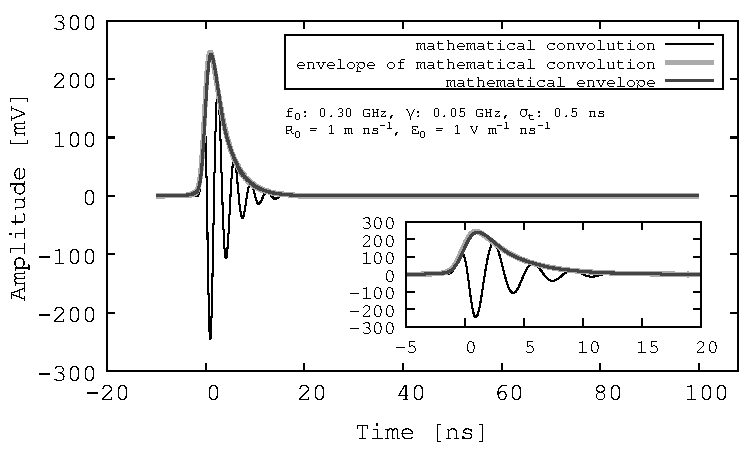
\includegraphics[width=0.5\textwidth]{July3rd_plot1.pdf}
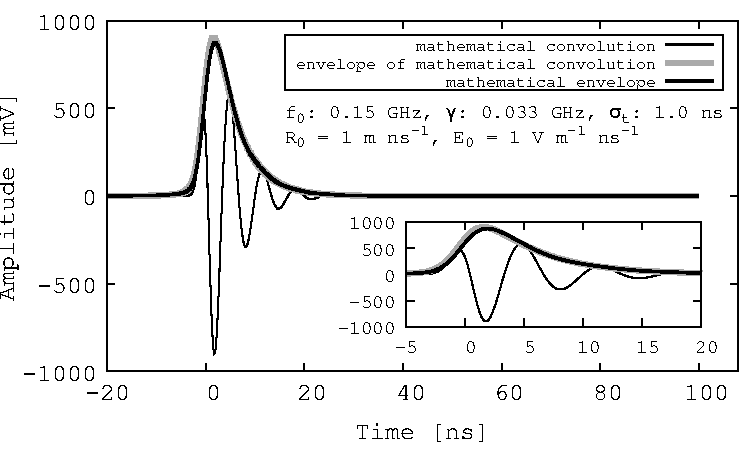
\includegraphics[width=0.5\textwidth]{July3rd_plot2.pdf}
\caption{\label{fig:fig1} (Top) The thin black line represents $s(t) * r(t)$.  The light gray envelope represents the envelope of $s(t) * r(t)$ computed with the Python3 SciPy function scipy.special.hilbert. The dark gray envelope represents Eq. \ref{eq:final}-\ref{eq:final2}. (Bottom) Same as top, for different parameter values.}
\end{figure}
\item To demonstrate that \textit{numerical convolution} of $s(t)$ and $r(t)$ produces the same results as the \textit{mathematical convolution} of $s(t)$ and $r(t)$ (Eq. \ref{eq:final3}), the corresponding waveforms are shown in Fig. \ref{fig:fig2}.
\begin{figure}[ht]
\centering
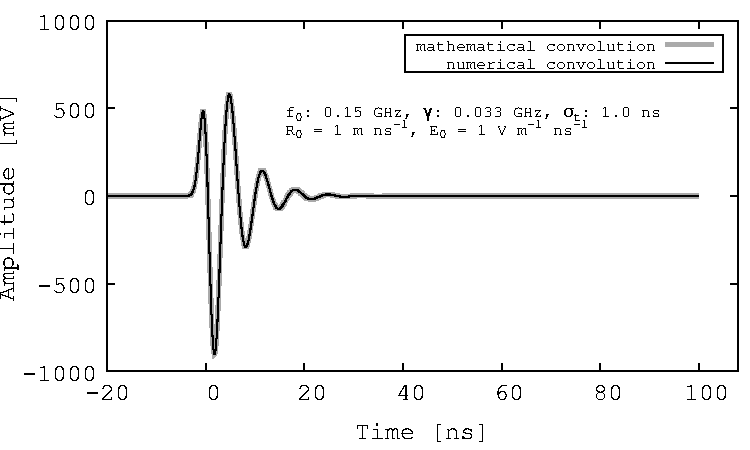
\includegraphics[width=0.5\textwidth]{July7th_plot1.pdf}
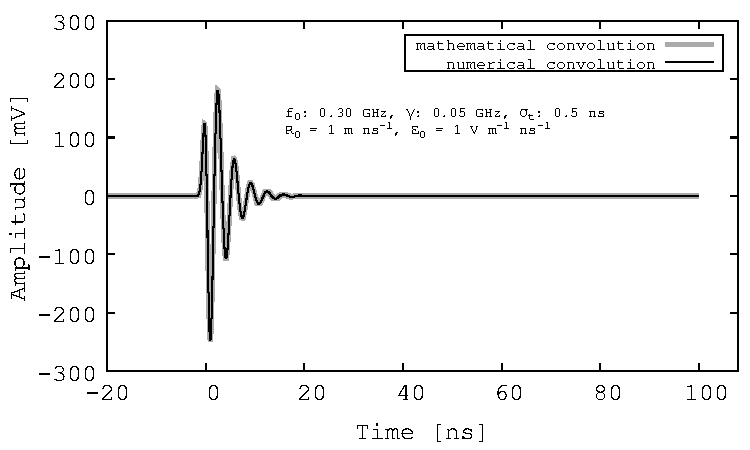
\includegraphics[width=0.5\textwidth]{July7th_plot2.pdf}
\caption{\label{fig:fig2} (Top) The thin black line represents $s(t) * r(t)$, produced using the Python3 SciPy function scipy.signal.convolve. The dark gray line represents Eq. \ref{eq:final3}. (Bottom) Same as top, for different parameter values.}
\end{figure}

\item A Monte Carlo data set was generated using NuRadioMC for UHE-$\nu$ interactions in a cylindrical ice volume with a depth of 0.65 km and a radius of 0.85 km.  The UHE-$\nu$ energies ranged from 10-100 PeV, with roughly equal numbers of UHE-$\nu$ in each 10 PeV bin.  The detector had one string of 8 RF dipole antennas.  Each RF channel had a filtered, amplified passpand of [80,1000] MHz, with 256 samples per channel at a 1 GHz sampling rate.  The RF trigger responded when 3 of the 8 voltage traces exceeded $\pm 3$ times the $v_{\rm rms}$ of the thermal noise within 256 ns.  For each signal, the Hilbert envelope of the coherently summed waveform (CSW) was calculated and correlated against Eqs. \ref{eq:final}-\ref{eq:final2}.  A quick optimization over the whole data set yielded 0.15 GHz and 0.025 GHz for the $f_0$ and $\gamma$ parameters, respectively.  Each correlation was maximized by varying the just the $\sigma_t$ parameter, yielding an optimized analytical envelope for each event.  A thermal noise waveform reflective of the channel properties was also generated for each event.  The noise waveform was also correlated against the optimized analytical envelope.  Both correlation distributions are shown in Fig. \ref{fig:fig3}.

\begin{figure}
\centering
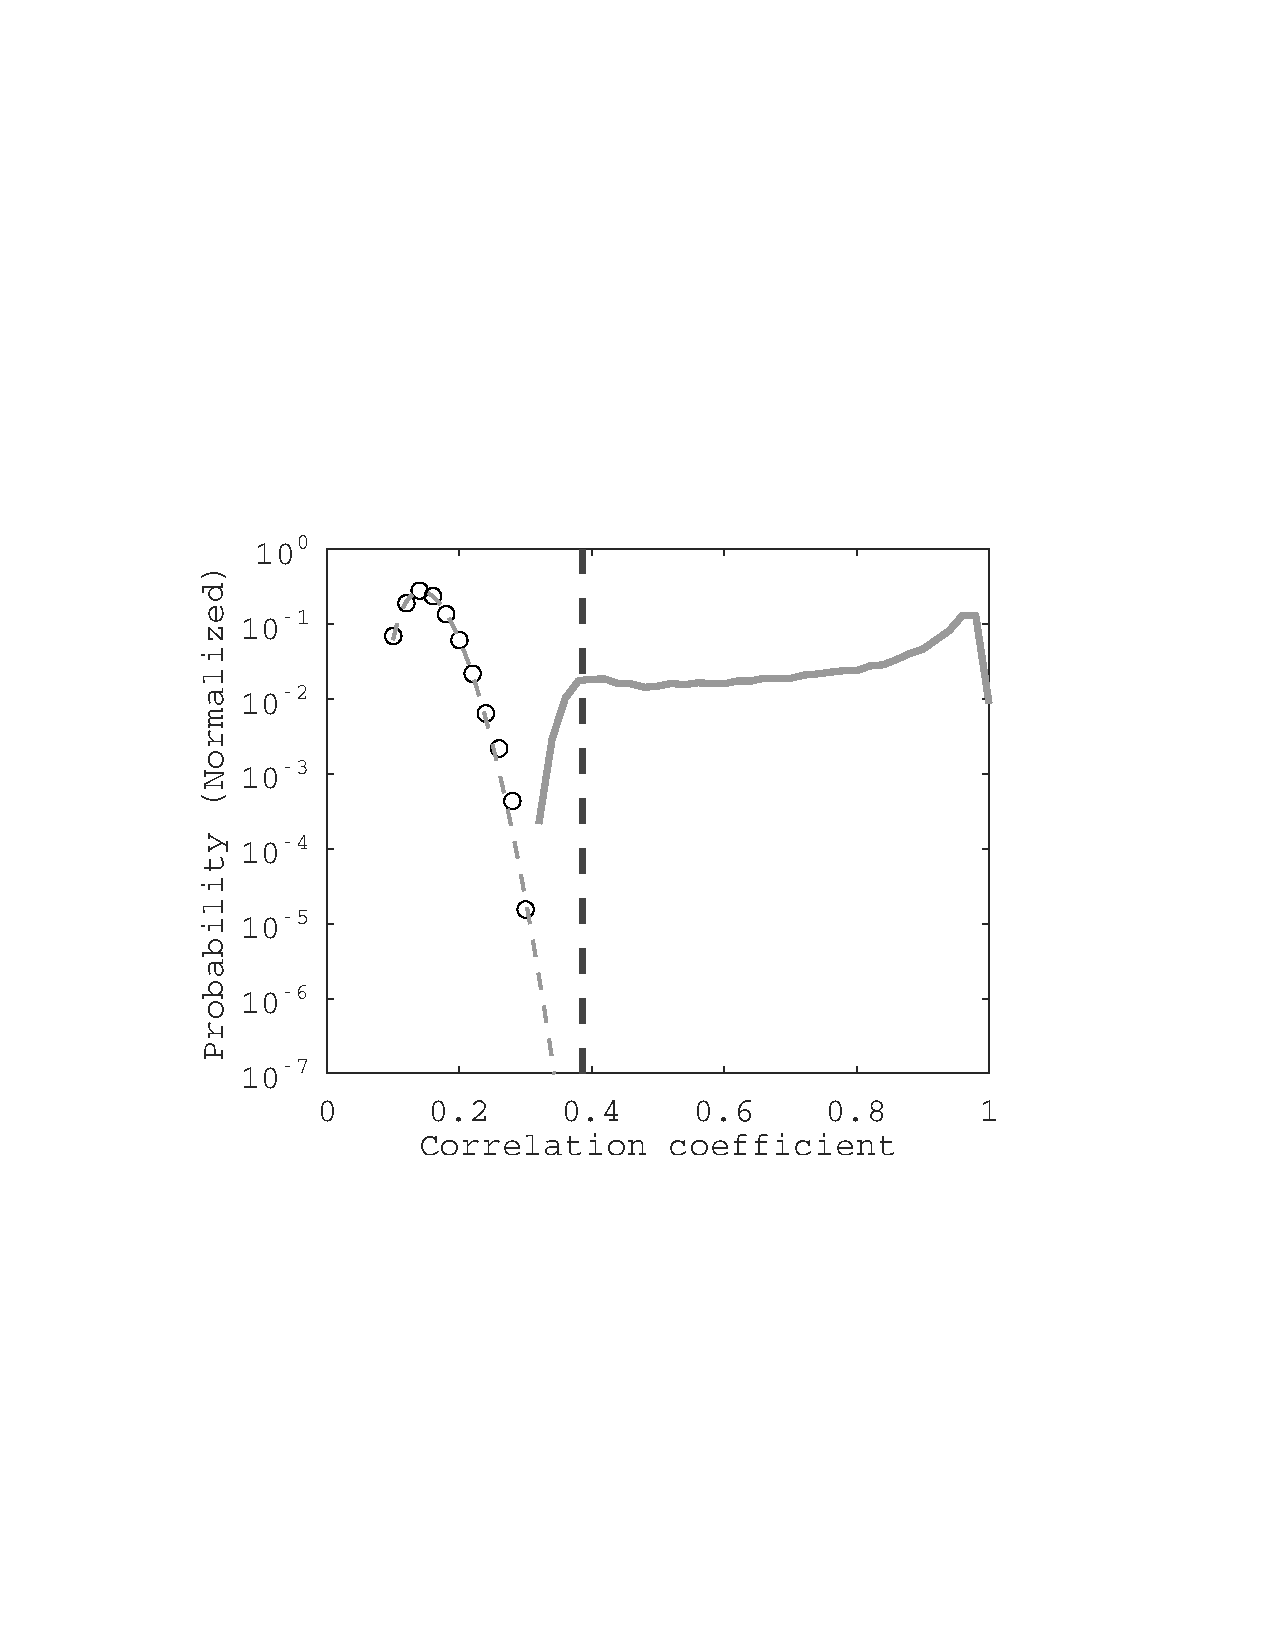
\includegraphics[width=0.5\textwidth,trim=3.25cm 8.25cm 4.5cm 9.0cm,clip=true]{Aug15_plot1.pdf}
\caption{\label{fig:fig3} (Black circles) Noise distribution. (Gray dashed line) Fitting function to noise distribution.  (Solid black line) Exponential fit to tail of noise distribution.  (Solid gray line) UHE-$\nu$ signal distribution.  (Dashed black line) Optimized correlation coefficient threshold value.}
\end{figure}

In Fig. \ref{fig:fig3}, the circles represent the normalized histogram of the correlation coefficent between the optimized analytic envelope and the thermal noise.  Functions of the forms $x^2 \exp(-0.5 x^2)$ and $\exp(-x)$ were fit to the noise distribution on the intervals [0.1,1.0] and [0.28,1], respectively.  The former is represented by the gray dashed line, and the latter is represented by the solid black line.  The solid gray line represents the signal distribution, which peaks at a correlation value of 0.96.  The vertical black dashed line represents a threshold of 0.438.  For the simulated UHE-$\nu$, 92\% of correlations between CSWs and optimized analytic envelopes are greater than or equal to this threshold.  Assuming the solid black line describes the noise distribution tail, with a noise trigger rate of 1 Hz, the threshold is equivalent to 0.95 noise events every 5 years.

\begin{figure}
\centering
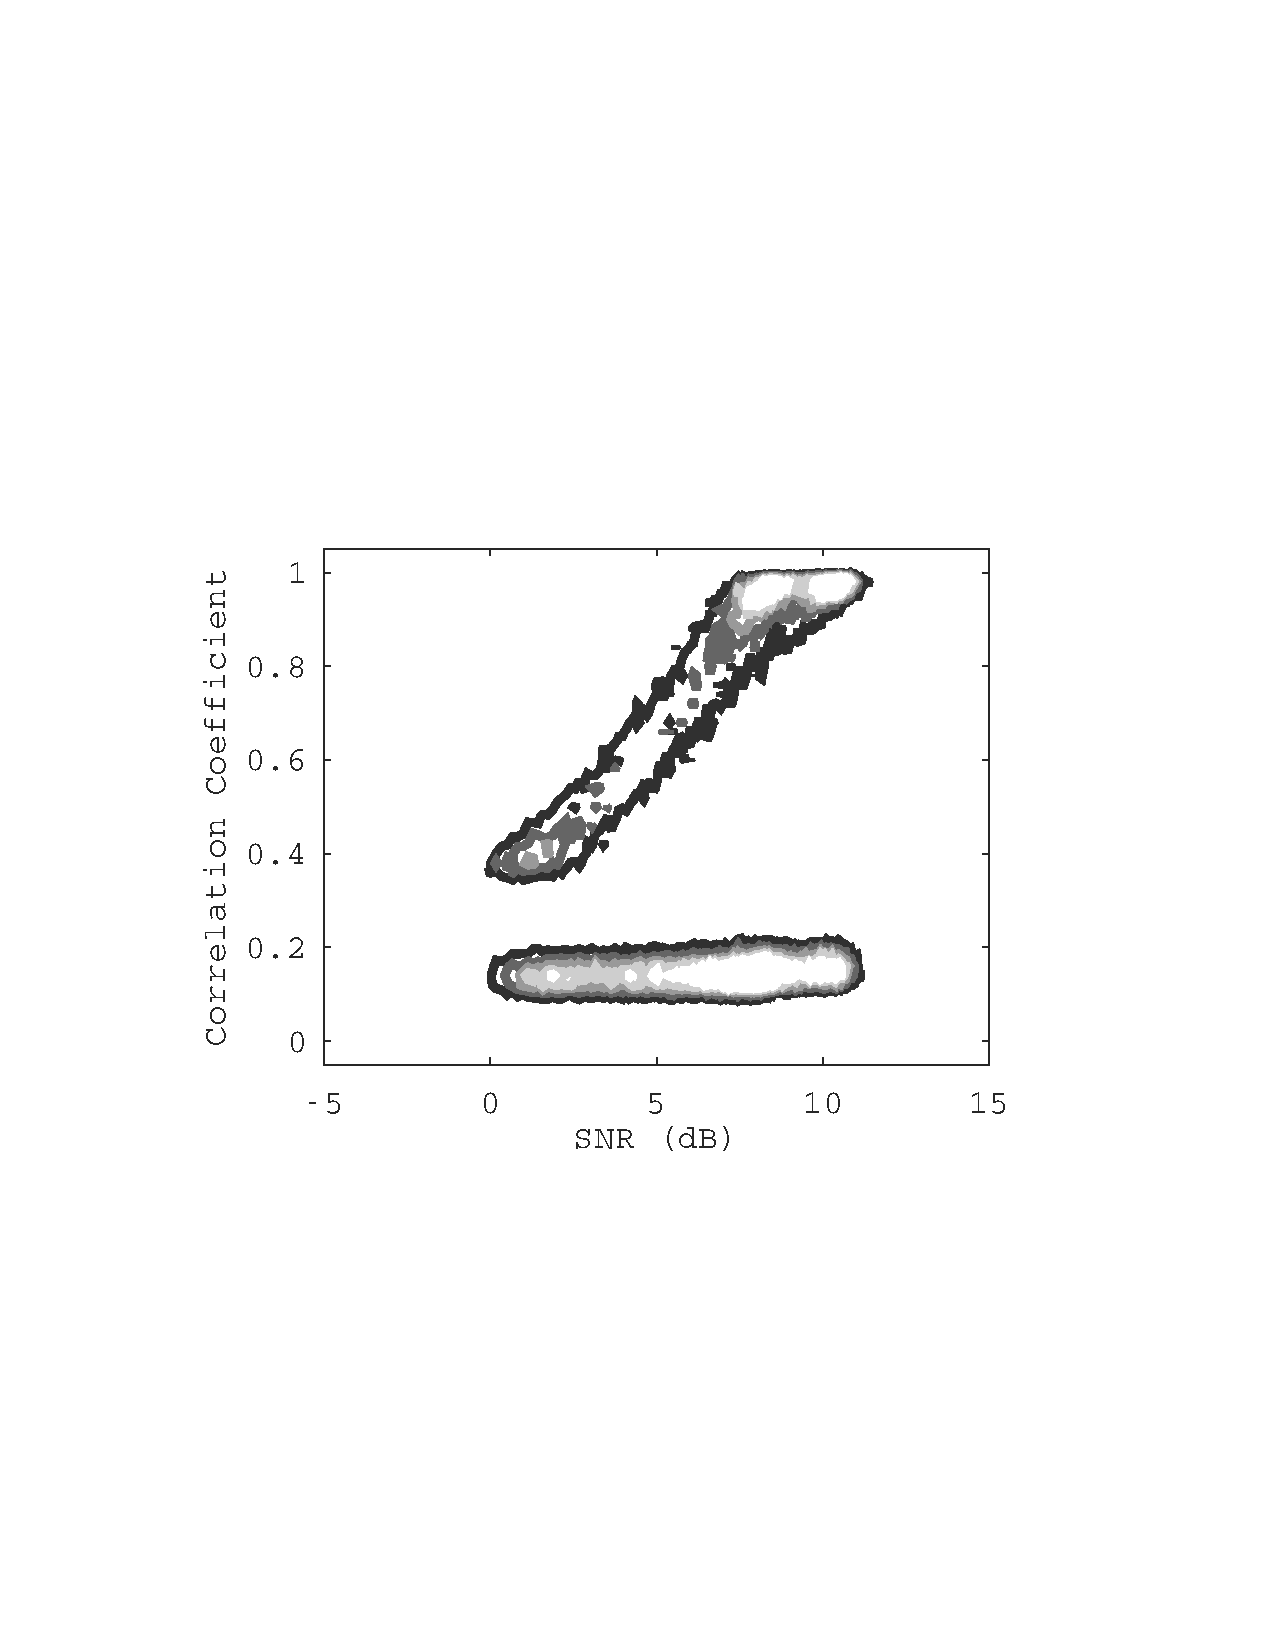
\includegraphics[width=0.5\textwidth,trim=3.25cm 8.25cm 4.5cm 9.0cm,clip=true]{Aug15_plot2.pdf}
\caption{\label{fig:fig4} The correlation versus SNR (dB) for UHE-$\nu$ signals (upper distribution) and RF thermal noise (lower distribution).  Color scale: normalized histogram value, with five equally spaced contours between 0.0 and 0.003.}
\end{figure}

The correlation between the optimized analytical envelope and UHE-$\nu$ signals depends on the signal to noise ratio (SNR).  Let $v_{\rm pp}$ and $v_{\rm rms}$ represent the peak-to-peak and rms values a voltage traces, respectively.  The SNR, in decibels, is defined as

\begin{equation}
\snr_{\rm dB} = 20\log_{10}\left(\frac{1}{2}\frac{v_{\rm pp}}{v_{\rm rms}}\right)
\end{equation}

In Fig. \ref{fig:fig4}, the correlation coefficient is plotted versus the SNR in dB for the data shown in Fig. \ref{fig:fig3}.  The upper distribution corresponds to CSWs from UHE-$\nu$ events, and the flat distribution corresponds to the CSWs from RF thermal noise.  UHE-$\nu$ events with SNR values $>5$ dB tend to maximize the correlation coefficient, and the correlation coefficient decreases linearly with decreasing SNR (dB).  As expected, the correlation coefficient for thermal noise does not depend on SNR, since the thermal fluctuations that increase the SNR do not resemble the optimized analytic envelope.  Note that the SNR of a CSW does not equal the SNR of the individual voltage traces.  Rather, the individual voltage traces will have SNR values approximately 5-10 dB \textit{lower} than the CSW SNR.  If $N$ voltage traces contain signal, computing the CSW raises the linear SNR by a factor of $\sqrt{N}$, and adds to the SNR in dB a factor of $20\log_{10}(N)$.  For an event with 3 of 8 channels containing signal, $20\log_{10}(3)\approx 5$ dB, while $20\log_{10}(8)\approx 9$ dB.  The exact increase in SNR from traces to CSW depends on how many RF channels contain significant signal.

\begin{figure}
\centering
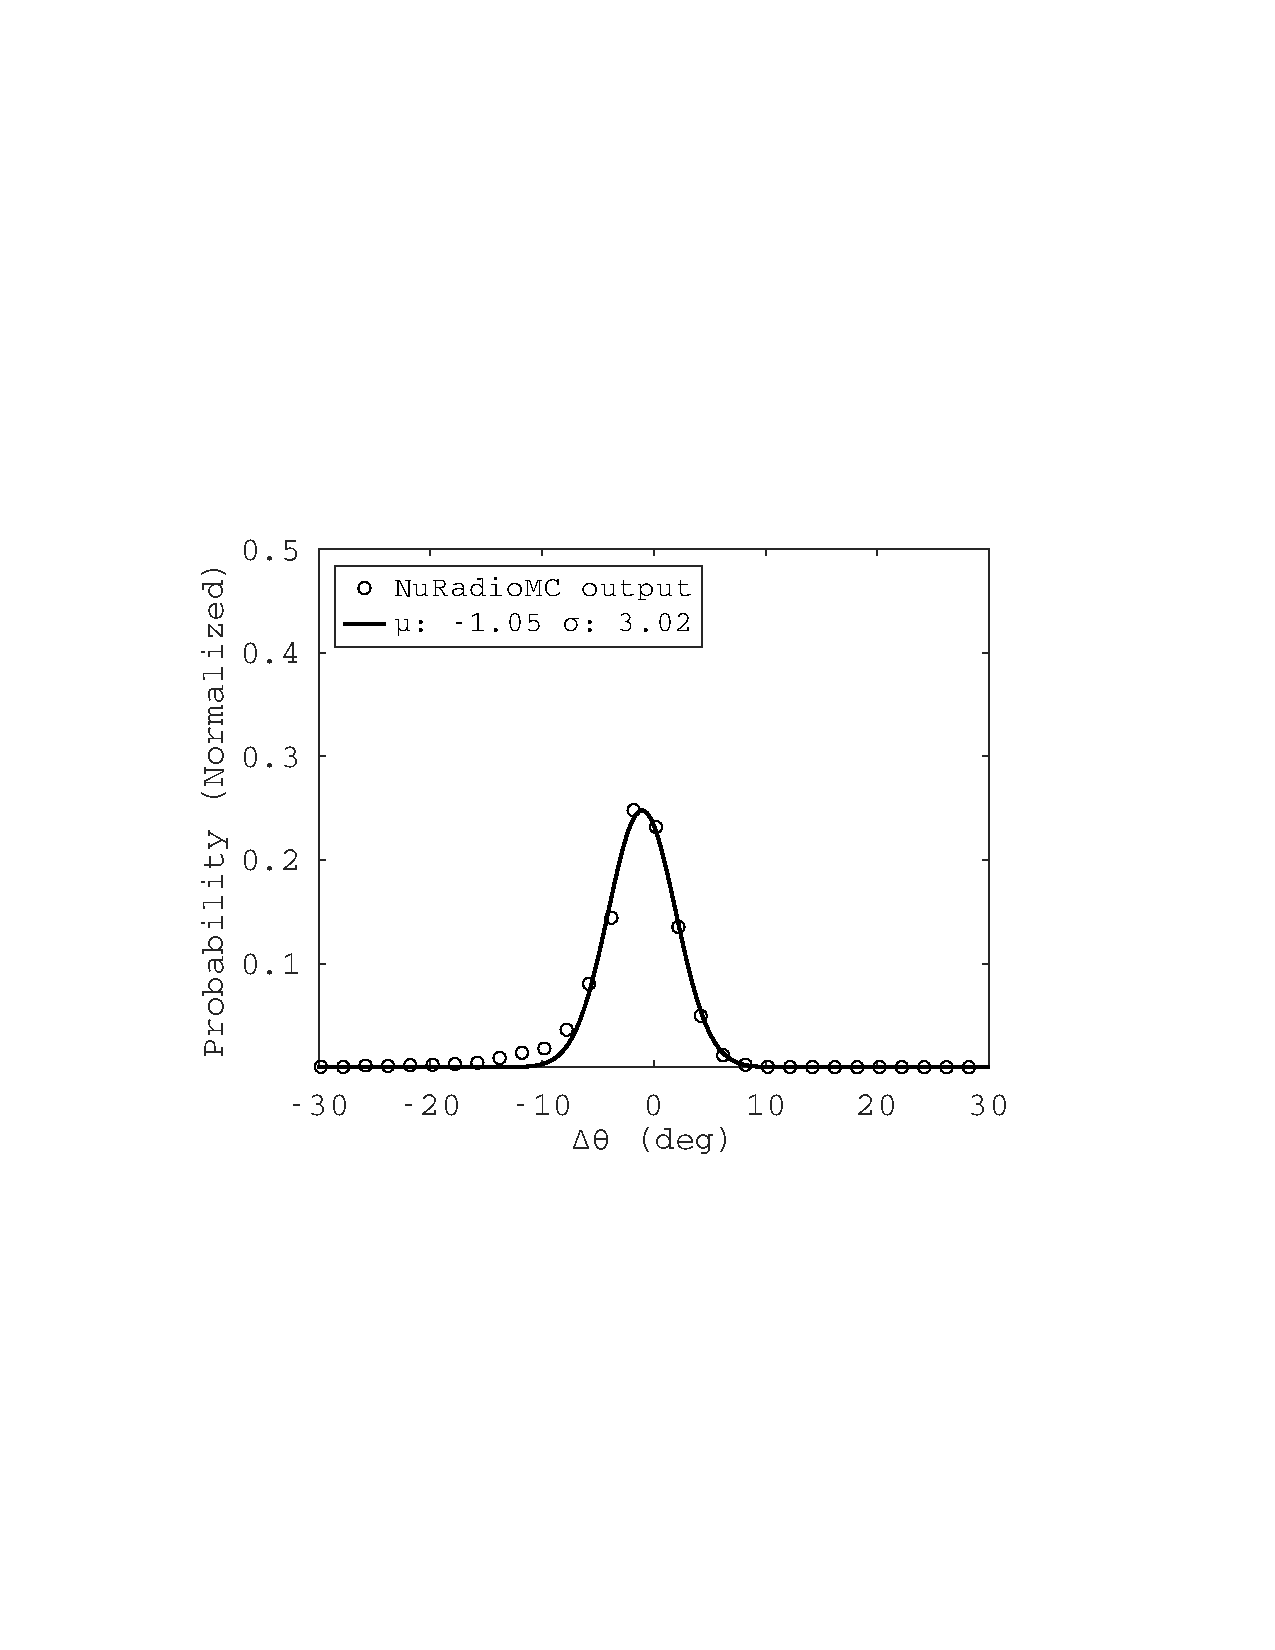
\includegraphics[width=0.5\textwidth,trim=3.25cm 8.25cm 4.5cm 9.0cm,clip=true]{Aug18_plot1.pdf}
\caption{\label{fig:fig5} (Black circles) Viewing angle from NuRadioMC. (Solid black line) Gaussian fit, with $\mu = 55.6$ deg, and $\sigma = 5.77$ deg.  (Black dashed line) Cherenkov angle, $\theta_{\rm C}$.}
\end{figure}

\item Equations \ref{eq:uncert}-\ref{eq:a_err} may be used to reconstruct the natural logarithm of the UHE-$\nu$ cascade energy, $\ln\Lambda$.  For Eq. \ref{eq:uncert}, $\sigma_t$ is measured from the optimized analytic envelope, $c$ and $\theta_{\rm C}$ are known constants, and an assumption must be made for $\Delta\theta$.  We will make the assumption that $\Delta\theta \approx \Delta\theta_{\rm rms}$.  Relying on a single string of RF channels makes calculating $\Delta\theta$ difficult, and geometric event reconstruction usually requires interferometry with multiple strings (cite).  However, the assumption is justified since the $\Delta\theta$ distribution is Gaussian.  The MC truth for $\Delta\theta$ in this analysis is shown in Fig. \ref{fig:fig5}, with a Gaussian fit ($\mu=55.6$ deg, $\sigma=5.77$ deg).  The rms and the $\sigma$ parameter are identical for Gaussian distributions, so we assume $\Delta\theta \approx 5.77$ deg.  The fractional error $\sigma_{\Delta\theta}/\Delta\theta$ is then set to 1.0, reflecting our uncertainty in this parameter.  Solving Eq. \ref{eq:uncert} for $a$ gives

\begin{equation}
a = \frac{c\sigma_t}{\Delta\theta_{\rm rms} \sin\theta_{\rm C}}
\end{equation}

The result for the fractional error in $a$ is found by propagating error from $\sigma_t$ and $\Delta\theta$, defined as $\epsilon$ and $\sigma_{\Delta\theta}$, respectively.  The result is

\begin{equation}
\frac{\sigma_a}{a} = \left(\left(\frac{\epsilon}{\sigma_t}\right)^2 +  \left(\frac{\sigma_{\Delta\theta}}{\Delta\theta}\right)^2\right)^{1/2}
\end{equation}

The first term is small compared to the second, as it is limited by the scan resolution for $\sigma_t$ in the optimization of the analytic envelope and the number of samples per envelope.  The scan resolution is set to 50 ps in the optimization, and there are typically $>10$ samples per envelope.  Thus, the main source of error is $\sigma_{\Delta\theta}$, and

\begin{equation}
\frac{\sigma_a}{a} = \left|\frac{\sigma_{\Delta\theta}}{\Delta\theta}\right| = \left|\frac{\Delta\theta_{\rm rms}}{\Delta\theta_{\rm rms}}\right|\approx 1
\end{equation}

Setting the ratio to 1 reflects the idea that the rms is equal to $\sigma$ for a normal distribution.  Inserting this assumption into Eq. \ref{eq:a_err} gives

\begin{equation}
\frac{\sigma_{\ln\Lambda}}{\ln\Lambda} \approx 2 \label{eq:a_err_2}
\end{equation}

Using Eqs. \ref{eq:em} and \ref{eq:had}, the logarithm of the energy is

\begin{equation}
\ln\Lambda = \left( \frac{c\sigma_t}{c_{\rm em/had} \Delta\theta_{\rm rms}\sin\theta_{\rm C}} \right)^2 \label{eq:lnLambda}
\end{equation}

Using Eqs. 10 and 12 from HH (\cite{PhysRevD.105.123019}), $c_{\rm em}$ and $c_{\rm had}$ were found to be 0.80 and 0.93 meters, respectively (FWHM, $R=0.5$).  Using Eq. \ref{eq:lnLambda}, the $\sigma_t$ results from the optimized envelope fits to UHE-$\nu$ CSWs may be used to deduce the UHE-$\nu$ energy distribution.  Two modifications facilitate interpretation.  First, converting to the base-10 logarithm is more convenient, and this introduces a factor of $\ln(10)$ in the denominator of Eq. \ref{eq:lnLambda}.  Second, $\ln\Lambda = \ln(E_{\rm C}/E_{\rm crit})$, where $E_{\rm C}$ is the energy in the UHE-$\nu$ induced cascade, and $E_{\rm crit}\approx 10^8$ eV is known as the critical energy \cite{PhysRevD.105.123019}.  Since $\ln\Lambda = \ln E_{\rm C} - \ln E_{\rm crit}$, separating this ratio simply adds a constant to the right hand side of Eq. \ref{eq:lnLambda}.  The modified form of Eq. \ref{eq:lnLambda} is

\begin{equation}
\log_{10} E_{\rm C} = \frac{\left( \frac{c\sigma_t}{c_{\rm em/had} \Delta\theta_{\rm rms}\sin\theta_{\rm C}} \right)^2}{\ln 10} + \log_{10} E_{\rm crit} \label{eq:lnLambda_2}
\end{equation}

Figure \ref{fig:fig6} contains the $\sigma_t$ distribution, converted into $\log_{10} E_{\rm C}$.  Note that when applying the change of base formula, factors of $\ln(10)$ cancel in the ratio of Eq. \ref{eq:a_err_2}.  The histogram is spread out over a range much larger than the expected range from NuRadioMC.  However, the average value of the histogram is $15.7 \pm 4.5$, in agreement with the prediction from NuRadioMC and Eq. \ref{eq:a_err_2}: $16.7 \pm 2.0$.  Thus, the energy reconstruction produces the correct order of magnitude on average, if not the precise value.

\begin{figure}
\centering
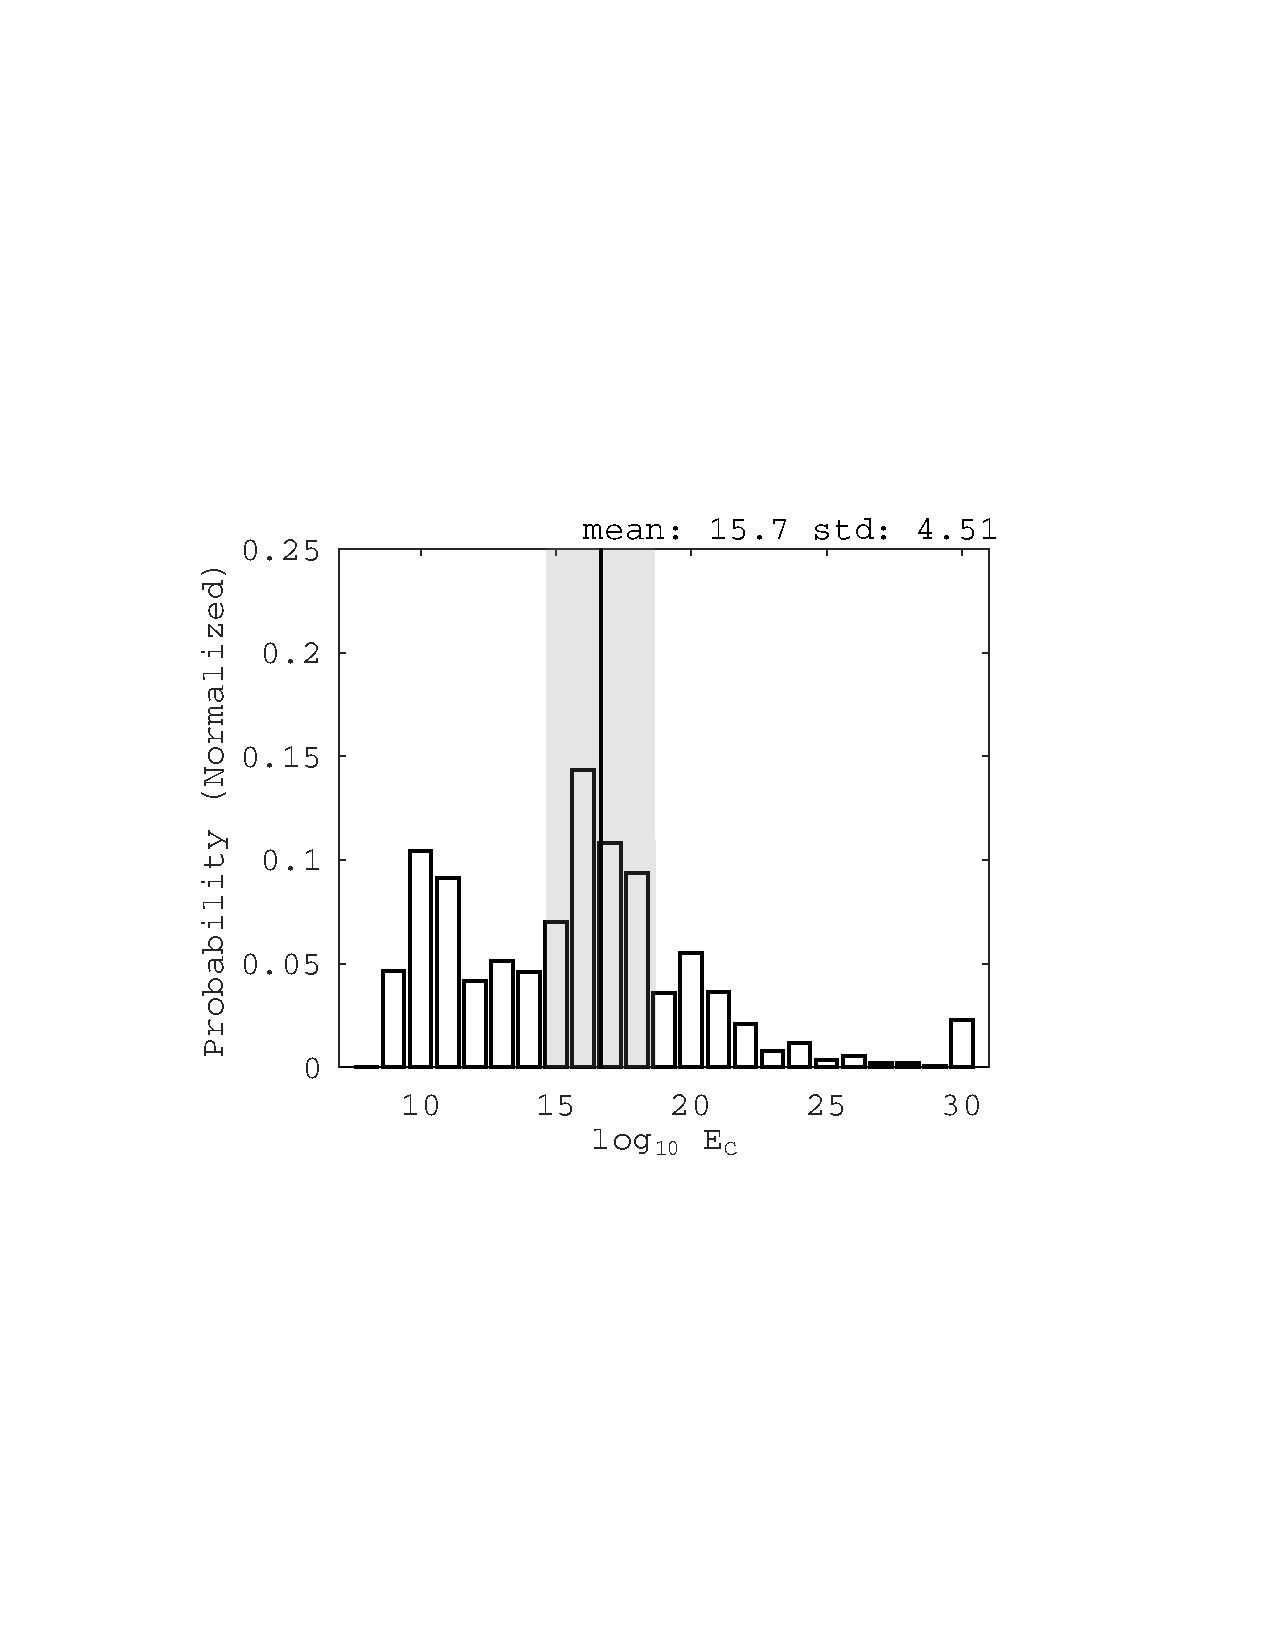
\includegraphics[width=0.5\textwidth,trim=3.25cm 8.25cm 4.5cm 8.25cm,clip=true]{Aug19_plot1.pdf}
\caption{\label{fig:fig6} Normalized distribution of $\sigma_t$ values, converted to $\log_{10}E_{\rm C}$ via Eq. \ref{eq:lnLambda_2}.  The vertical black line represents the average $\log_{10}E_{\rm C}$ from the NuRadioMC energies, and the shaded region represnts the $1\sigma$ error range using Eq. \ref{eq:a_err_2}.}
\end{figure}

\end{itemize}

\section{Conclusion}
\label{sec:conc}

The conclusion.

\appendix

\section{Details}
\label{app:a}

The details.

\bibliography{apssamp}

\end{document}

